\section{Experiments}

Our theory leads to algorithmic consequences of practical interest.
First, we show that the diagnosis metric that we proposed in Section \ref{sec_similarity} can help predict positive or negative transfer using only STL performances.
Second, \todo{}.
Finally, we validate the three components of our theory on image and text classification tasks.


\begin{table}
\begin{minipage}[t]{.58\textwidth}
	\centering
  \begin{tabular}{c c c c c}
	\toprule
		\multirow{2}{*}{{\bf Threshold}}  & \multicolumn{2}{c}{{\bf Text
		classification}} & \multicolumn{2}{c}{{\bf ChestX-ray14}} \\
		& Precision &  Recall & Precision &  Recall \\
		\cmidrule(lr){1-1} \cmidrule(lr){2-3} \cmidrule(lr){4-5}
		0.0 & 0.596 & 1.000 & 0.593 & 1.000 \\
		0.1 & 0.756 & 0.388 & 0.738 & 0.462 \\
		0.2 & 0.919 & 0.065 & 0.875 & 0.044 \\
		% 0.3 & 1.000 & 0.004 &     - &     - \\
	\bottomrule
	\end{tabular}
	\vspace{0.1in}
	\captionof{table}{Ablation study on when should use MTL via different source/target task accuracy.}
	\label{tab:mtl_better_than_stl}
\end{minipage}
\quad
% \vspace{}
\begin{minipage}[t]{.40\textwidth}
	\centering
	\begin{tabular}{c c c}
		\toprule
		\multirow{2}{*}{{\bf Models}} & \multicolumn{2}{c}{\begin{minipage}{1.1in}\begin{center}
		MR, SST, SUBJ, CR, MPQA, TREC\end{center}\end{minipage}} \\
		\cmidrule(lr){2-3}
		& {\bf Standard} & {\bf Alignment} \\
		\midrule
		{\bf MLP}  & > 100\% & 39\% \\
		{\bf LSTM} & 36\% & 36\% \\
		\bottomrule
		\end{tabular}
	\vspace{0.1in}
	\captionof{table}{Taskonomy experiment.}
	\label{tab:taskonomy}
\end{minipage}
\end{table}

\subsection{Experimental Setup}

{\bf Datasets and models.} We describe the datasets and models we use in the experiments.

{\it Sentiment Analysis:} This dataset includes six tasks: movie review sentiment (MR), sentence subjectivity (SUBJ), customer reviews polarity (CR), question type (TREC), opinion polarity (MPQA), and the Stanford sentiment treebank (SST) tasks.

{For each task, the goal is to categorize sentiment opinions expressed in the text.
We use an embedding layer (with GloVe embeddings\footnote{http://nlp.stanford.edu/data/wordvecs/glove.6B.zip}) followed by an LSTM layer proposed by~\cite{lei2018simple}.
}
%multi-layer perceptron (MLP), LSTM, CNN on all tasks
%We use this task to verify our theoretical results on model capacity and task covariance in real world.

{\it ChestX-ray14:} This dataset contains 112,120 frontal-view X-ray images and each image has up to 14 diseases.
This is a 14-task multi-label image classification problem.
%We treat each label as one task a binary classification problem and formulate it as a 14-task multi-task learning problem.
%This dataset is curated where the labels
%We use the CheXNet model from~\cite{chexnet}, which is a 121-layer convolutional neural network on all tasks.

For all models, we share the main module across all tasks and assign a separate regression or classification layer on top of the shared module for each tasks.



\subsection{Experimental Results}

\textbf{A single-task based diagnosis metric.}
We validate the metric proposed in Section \ref{sec_similarity} for predicting positive or negative transfer based on single-task accuracies.
Table \ref{tab:mtl_better_than_stl} shows the result on both the sentiment analysis and the ChestX-ray14 datasets.
We find that using a threshold of $0.1$, our predicts correctly predicts positive or negative transfer with $75.6\%$ accuracy among 150 task pairs with $38.8\%$ recall.
We observe similar results for 91 task pairs from the ChestX-ray14 dataset.
The result shows that STL performances are indicative for the diagnosis of MTL performances.

\textbf{Improving training efficiency via an incremental schedule.}
\todo{}

\textbf{MTL improves labeled data efficiency.}
We measure the data efficiency ratio on the sentiment analysis tasks.
We find that by performing multi-task learning, only $39\%$ of the labeled data is needed to achieve comparable performance to single-task learning over all six tasks.
If TREC is not included, we see that only $25\%$ of the labeled data is needed.


\subsection{Ablation Studies}


\textbf{Task similarity.} \todo{}


\textbf{Data size.}
Recall that Proposition \ref{prop_data_size} shows that increasing the data size of the source task does not always improve the performance of MTL for the target task.
In Figure \ref{fig_ab_data}, we observe that for the task pair MR and SST, increasing the data size of MR is helpful initially, but then gets worse.


\textbf{Covariate shift.}
Our result provides a fine-grained insight on the covariance alignment algorithm proposed in \cite{WZR20}.
Recall that the covariance alignment procedure in \cite{WZR20} adds an additional module between the word embedding representation and the shared module.
When the source task data size is particularly large compared to the target task, then we expect that applying the covariance alignment algorithm results in a more significant gain.
We validate that the performance of aligning task covariances depends on the size of source task data.
In Figure \ref{fig_ab_cov}, we observe that the benefit from aligning task covariances becomes more significant as we increase the size of the source task dataset.


\begin{figure}[!t]
	\centering
	\begin{subfigure}[b]{0.33\textwidth}
		\centering
		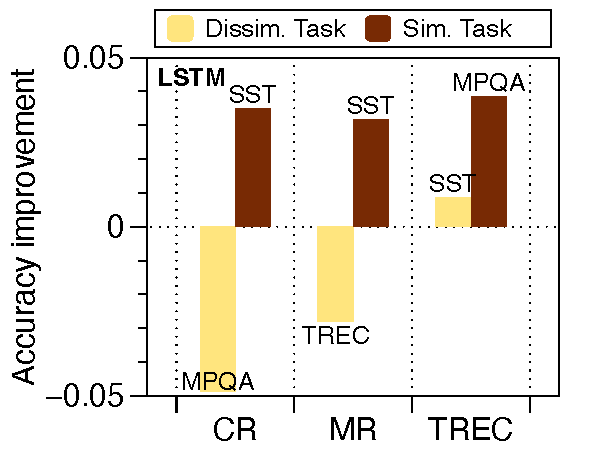
\includegraphics[width=0.975\textwidth]{figures/task_sim_norm_lstm.pdf}
		\caption{Task model}
		\label{fig_ab_sim}
	\end{subfigure}%
	\begin{subfigure}[b]{0.33\textwidth}
		\centering
		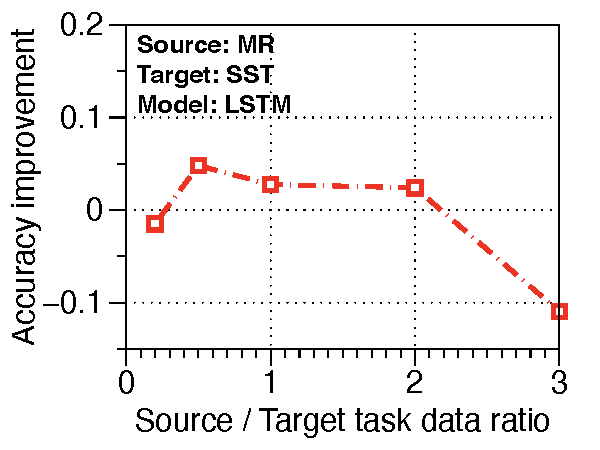
\includegraphics[width=0.975\textwidth]{figures/ratio_norm_sst_trec_lstm.pdf}
		\caption{Data size}
		\label{fig_ab_data}
	\end{subfigure}
	\begin{subfigure}[b]{0.33\textwidth}
		\centering
		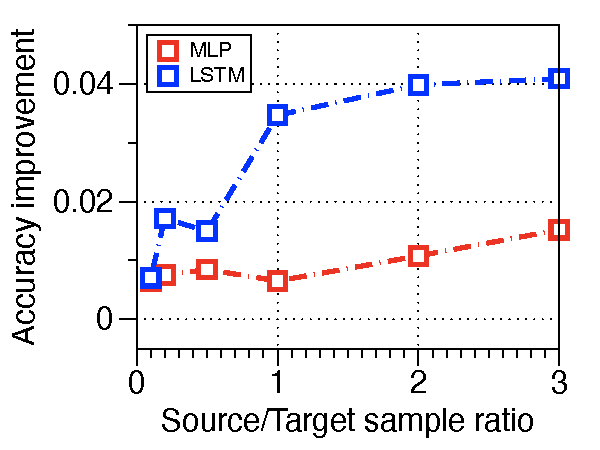
\includegraphics[width=0.975\textwidth]{figures/ratio_alignment_norm_diff_all.pdf}
		\caption{Covariate shift}
		\label{fig_ab_cov}
	\end{subfigure}
	\caption{The performance of aligning task covariances depends on data size. As the ratio between source task data size and target task data size increases, the performance improvement from aligning task covariances increases.}
	\label{fig_ablation}
\end{figure}

